%%
%% Kapitel:
%%
\chapter{Bilder mit PS}
\label{BilderPS}
%%======================================================================



\section{Bilder}

Etwas trickreich, da \LaTeX\ urspr�nglich daf�r nicht vorgesehen war.

\subsection{Postscript}
  
Die einfachste Variante benutzt \emph{Postscript}. Hat den Vorteil,
dass man CAD-Zeichnungen einfach einbinden kann. Beim Skalieren
werden die Strichbreiten auch skaliert. JPGs kann man mit
\texttt{jpeg2ps} in Postscript umwandeln.\\
Nachteil: Drucker muss Postscript k�nnen, \texttt{ghostscript} muss installiert sein!

\includegraphics[width=80mm]{0060/bild_ps.ps} 	      
          







